\documentclass[11pt,a4paper]{article}
\usepackage[T1]{fontenc}
\usepackage[utf8]{inputenc}
\usepackage{lmodern,microtype}
\usepackage{amsmath,amssymb,amsthm,mathtools,bm}
\usepackage{booktabs,array,tabularx,longtable}
\usepackage{graphicx,float,caption}
\usepackage{xcolor}
\usepackage[margin=20mm]{geometry}
\usepackage{enumitem}
\usepackage{fancyhdr}
\usepackage[hidelinks]{hyperref}
\hypersetup{
  pdftitle={FIN ST16--ST27: Selectors, Refinement, and the Dimensional Bridge},
  pdfauthor={Krzysztof Żuchowski},
  pdfsubject={Local analytical and computational execution of programs ST16--ST27},
  pdfkeywords={FIN, spectral operator, Jordan chain, Krein stability, refinement, gauge connection, dimensional equivariance}
}
\setlength{\parindent}{0pt}
\setlength{\parskip}{0.50em}
\setlength{\emergencystretch}{2em}
\setlength{\headheight}{14pt}
\setlist[itemize]{leftmargin=1.55em,itemsep=0.16em,topsep=0.2em}
\setlist[enumerate]{leftmargin=1.75em,itemsep=0.16em,topsep=0.2em}
\pagestyle{fancy}
\fancyhf{}
\lhead{FIN ST16--ST27}
\rhead{Release 10.56}
\cfoot{\thepage}
\newtheorem{theorem}{Theorem}[section]
\newtheorem{proposition}[theorem]{Proposition}
\newtheorem{corollary}[theorem]{Corollary}
\newcommand{\proven}{\textcolor{green!40!black}{\textbf{[PROVEN]}}}
\newcommand{\strong}{\textcolor{blue!70!black}{\textbf{[STRONG EVIDENCE]}}}
\newcommand{\conditional}{\textcolor{black!60}{\textbf{[CONDITIONAL]}}}
\newcommand{\blocked}{\textcolor{red!72!black}{\textbf{[BLOCKED]}}}
\newcommand{\boundary}{\textcolor{orange!80!black}{\textbf{[BOUNDARY]}}}
\newcommand{\resultbox}[1]{\begin{center}\fcolorbox{blue!60!black}{blue!4}{\parbox{0.92\textwidth}{#1}}\end{center}}

\begin{document}

\pagenumbering{gobble}
\begin{titlepage}
\centering
\vspace*{1.45cm}
{\LARGE\bfseries FIN ST16--ST27\par}
\vspace{0.38cm}
{\Large Selectors, Refinement, and the Dimensional Bridge\par}
\vspace{0.45cm}
{\large Jordan-chain reduction, invariant-algebra obstructions, exact refinement fibers, locality bounds, and adversarial tests\par}
\vspace{1.20cm}
{\Large Krzysztof Żuchowski\par}
\vspace{0.24cm}
{\large Independent Researcher --- Fractal Information Theory Project\par}
{\large ORCID: 0009-0002-0909-3613\par}
\vspace{1.00cm}
{\large FIN Release 10.56 --- Version 1.0.0\par}
{\large August 10, 2026\par}
\vfill
\begin{minipage}{0.88\textwidth}
\textbf{Scope.} This report executes the twelve local programs ST16--ST27 recommended by Release 10.55. It studies the current finite strict operator and explicitly declared conditional extensions. It does not assume that FIN is a physical theory or a Theory of Everything.\par
\textbf{Method.} Exact finite-dimensional reductions, symbolic rank arguments, interval scalar arithmetic, deterministic numerical continuation, synthetic preregistration, negative controls, and fifteen live acceptance tests are included.\par
\textbf{Epistemic rule.} An exact theorem about a supplied model is not described as a derivation of that model from FIN. Binary64 collision locations, synthetic holdouts, and an unreplayed Lean source retain explicit boundaries.\par
\textbf{Repository.} \url{https://github.com/hyconiek/Fractal-Nadsoliton-Theory}\par
\textbf{License.} CC BY 4.0.
\end{minipage}
\end{titlepage}
\pagenumbering{arabic}

\begin{abstract}
Programs ST16--ST27 substantially sharpen the mathematical boundary between the finite strict FIN operator and a possible physical theory.

ST16 reduces the sampled Hamiltonian-memory transition to an explicit zero-mode Jordan-chain condition. If $v_0$ is the gauge vector and $Jv_1=v_0$, the collision occurs when $(J_0v_0)^Tv_1=0$. Eliminating the hidden blocks gives a quadratic polynomial in inverse mediator speed. The declared branch has one positive numerical root
\[
s_*=1.278014751820449,
\]
with full-block and reduced-scalar discrepancy below $2.9\times10^{-15}$. This identifies the transition mechanism but does not interval-certify the stationary state or $s_*$.

ST17 proves that every real symmetric operator natural under the full stabilizer of the strict $C_{12}$ geometry lies in the seven-dimensional radial algebra already equal to $C^*(A)$. Such generators cannot produce $M_{12}(\mathbb C)$ or solve the selector obstruction. ST18 constructs an infinite family of positive translation-invariant $C_{24}$ Laplacians satisfying the exact coarse intertwining relation $A_{24}(q)J=JA_{12}$. The free fine antipodal weight $q\ge0$ changes the unresolved modes, proving that positivity, cyclic covariance, and exact intertwining still do not select a unique refinement.

ST19 replaces the defining-kernel fingerprint by the derived mixed-channel identity $U_tP_\tau=\exp[-(\tau+it)A]$. A hashed synthetic holdout accepts every common-generator case and rejects every declared altered-unitary case, but supplies no physical record. ST20 interval-encloses the strict scalar spectrum, leaving a distinct-eigenvalue gap above $0.0435$ and positive unitary and wave branch margins above $2.0$. ST21 proves a finite-range path-order bound and a Duhamel truncation bound; the literal long-range continuation remains signed from distance eight.

ST22 compresses the operational obligations into five irreducible groups relative to finite operational-process semantics. ST23 proves that a continuous translation-invariant antisymmetric $U(1)$ one-form fixed by reflection must vanish. A nonzero oriented connection cannot be a deterministic stabilizer-equivariant function of $A$ alone. ST24 classifies a family of nonlinear mediator saturations: coercivity is controlled by a sharp asymptotic exponent threshold $a=1/2$. ST25 exports a Lean source but correctly remains blocked because no toolchain is configured. ST26 proves that the five spectral channels carry different positive-scaling weights, preventing a single dimension assignment to $A$. ST27 shows that isospectral sector-specific refits pass eigenvalue-only tests while a frozen matrix-level protocol rejects them.

No selector, unit, continuum, connection, apparatus, laboratory record, legacy-to-strict completion, or physical unification is obtained. The strongest advance is a collection of exact obstruction theorems and one analytically reduced stability mechanism.
\end{abstract}

\textbf{Status vocabulary.} \proven{} denotes an analytic identity or deterministic finite theorem in the declared model. \strong{} denotes robust non-interval numerical evidence. \conditional{} denotes a theorem after supplying named premises. \blocked{} marks an attempted deliverable that could not be completed. \boundary{} states the exact limit of an accepted result.

\tableofcontents
\newpage

\section{Starting object and outcome matrix}

The frozen strict object is
\[
W_{xx}=0,\qquad W_{xy}=\frac{\cos(0.18575d(x,y)+0.16250)}{1+d(x,y)^{1.8}}\quad(x\ne y),
\qquad A=sI-W\succeq0.
\]
The programs neither replace the strict kernel by the legacy kernel nor transfer historical legacy physical roles. The P530 memory realization, the ST08 link receiver, and the ST09 mediator are conditional extensions whose sources remain open.

\small
\begin{longtable}{@{}p{0.07\textwidth}p{0.31\textwidth}p{0.20\textwidth}p{0.33\textwidth}@{}}
\toprule
ID & Research object & Outcome & Principal boundary\\
\midrule
\endfirsthead
\toprule
ID & Research object & Outcome & Principal boundary\\
\midrule
\endhead
ST16 & Gauge-Jordan collision reduction & \proven{} $+$ \strong{} & Collision speed is not interval certified\\
ST17 & Stabilizer-natural algebra no-go & \proven{} & State-dependent breaking remains possible\\
ST18 & Exact positive refinement fiber & \proven{} & No internally selected functor\\
ST19 & Mixed-channel preregistration & \proven{} & Synthetic record and local custody\\
ST20 & Scalar-branch interval certificate & \conditional{} & Trusts \texttt{mpmath.iv} transcendental arithmetic\\
ST21 & Locality and tail bounds & \proven{} & Literal continuation is non-Markov\\
ST22 & Operational-obligation minimality & \proven{} & Relative to finite operational semantics\\
ST23 & Continuous connection-source no-go & \proven{} & State/boundary/$\pi$ sectors remain open\\
ST24 & Saturation universality classes & \proven{} & Constructed nonlinear family\\
ST25 & Proof-assistant replay & \blocked{} & Lean toolchain is not configured\\
ST26 & Dimensional equivariance & \proven{} & Does not select physical scales\\
ST27 & Isospectral adversarial refits & \proven{} $+$ \strong{} & Synthetic adversaries and threshold\\
\bottomrule
\end{longtable}
\normalsize

\section{ST16 --- Zero-mode Jordan-chain reduction}

Let $R_j=(A+c_jI)^{-1}$ for the supplied positive memory poles and let $u$ be the full-loading stationary state. The hidden Hamiltonian Jacobian has the exact block form
\[
J=J_0L,\qquad L=L^T.
\]
Its gauge vector $v_0$ can be written explicitly: the physical $y$ block is $u$, and hidden $b_j$ blocks are
\[
(v_0)_{b_j}=\sqrt{\frac{r_j}{s}}R_ju.
\]
The computed gauge residual is below $8.4\times10^{-16}$.

Let
\[
L_+=A+I-3\operatorname{diag}(u^2)+M,
\quad T=\sum_jr_jR_j^2,
\quad S=\sum_jr_jR_j^3.
\]

\begin{theorem}[Jordan-chain collision criterion]
Suppose $L_+$ is invertible. The equation $Jv_1=v_0$ is solvable. The zero Jordan chain extends by one further vector precisely when
\[
\kappa(s)=(J_0v_0)^Tv_1=0.
\]
After eliminating the hidden variables,
\[
\kappa(s)=-\left(c_0+\frac{2c_1}{s}+\frac{c_2+c_3}{s^2}\right),
\]
where
\[
c_0=\langle u,L_+^{-1}u\rangle,
\quad c_1=\langle u,L_+^{-1}Tu\rangle,
\quad c_2=\langle Tu,L_+^{-1}Tu\rangle,
\quad c_3=\langle u,Su\rangle.
\]
\end{theorem}

For the declared binary64 stationary state, the polynomial coefficients in $x=1/s$ are
\[
0.267156520118624\,x^2+0.112217945184788\,x-0.251372836109403.
\]
It has one positive-speed root $s_*=1.278014751820449$. At $s_*-10^{-4}$ the active spectrum has one positive real root with spectral abscissa $0.0065772$. At $s_*+10^{-4}$ the active spectral abscissa is below $1.2\times10^{-12}$. The reduced formula and the full generalized-chain calculation agree to $2.84\times10^{-15}$.

\begin{figure}[H]
\centering
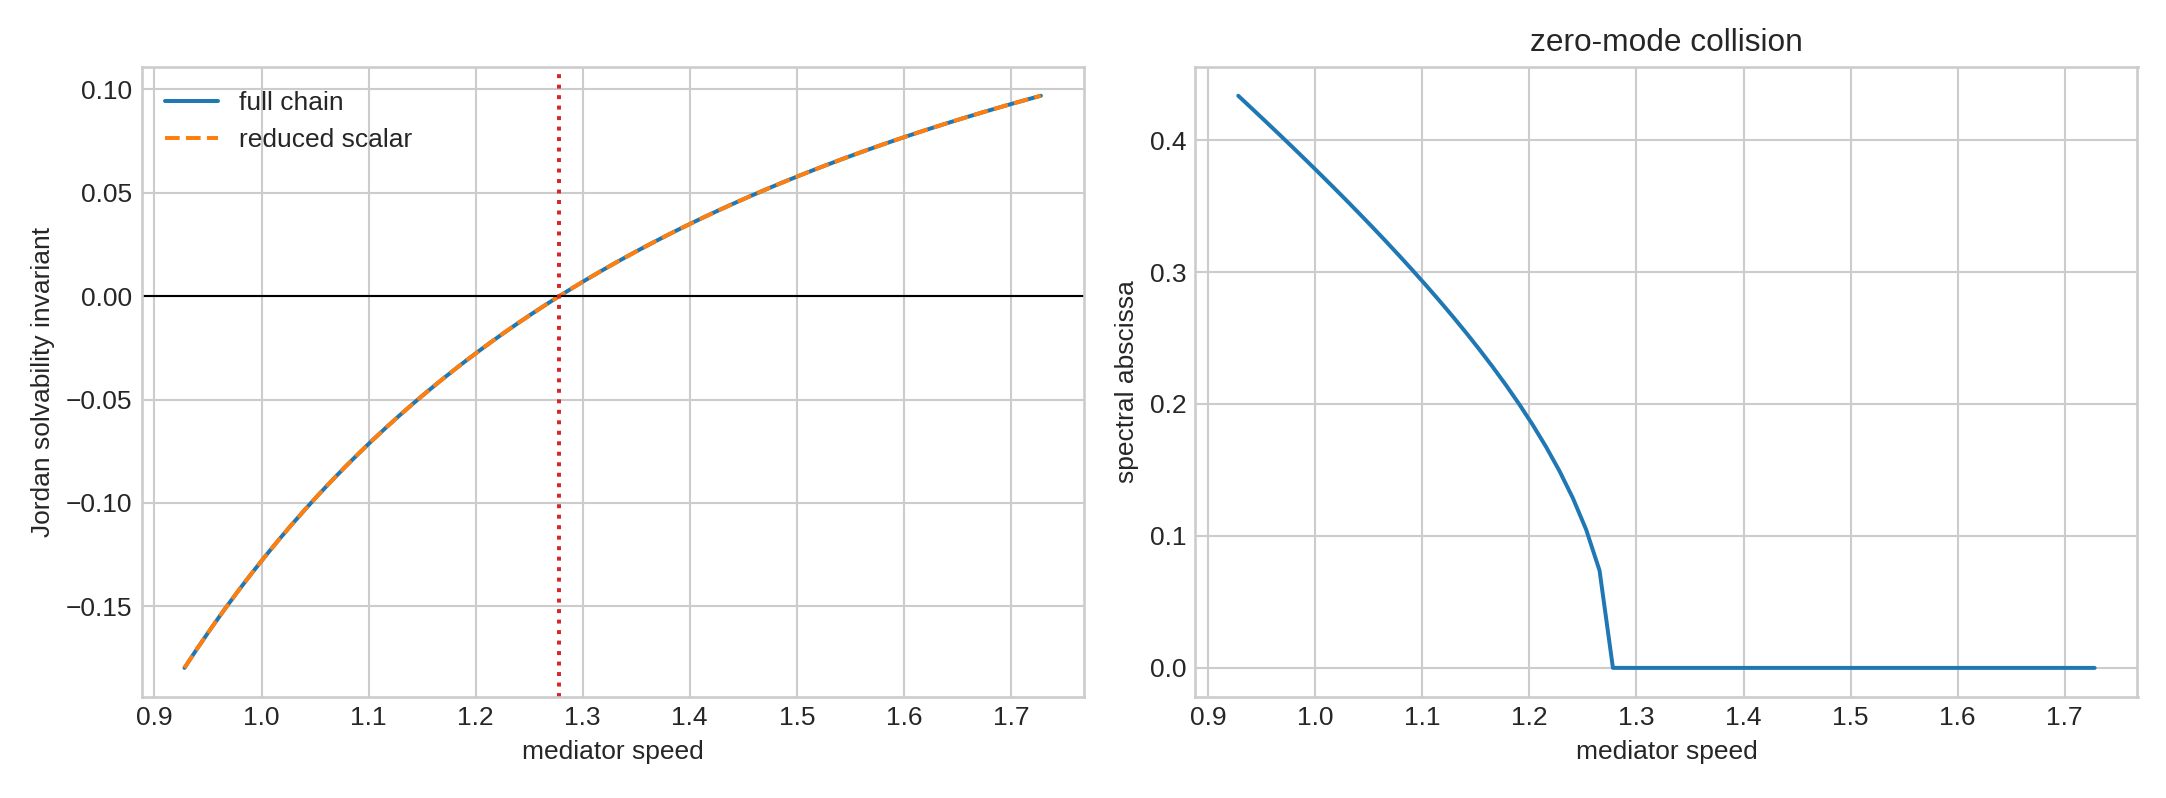
\includegraphics[width=0.94\textwidth]{FIN_ST16_ST27_Figures/st16_jordan_collision.png}
\caption{The reduced Jordan solvability invariant and the full-block calculation. The root identifies the numerical real-to-imaginary collision seen in ST10.}
\end{figure}

\boundary{} The algebraic reduction is exact for the declared block family. The coefficients use a non-interval stationary solution, so $s_*$ is strong numerical evidence rather than a proof-grade exact constant. This is not a global Krein-stability theorem.

\section{ST17 --- Selector-free invariant-algebra no-go}

The real symmetric matrices invariant under translations and reflection of $C_{12}$ are precisely radial circulants
\[
B_{xy}=b_{d(x,y)}.
\]
Their vector-space dimension is seven.

\begin{theorem}[Stabilizer-natural generator obstruction]
Strict $A$ has seven distinct spectral values, so $C^*(A)$ has dimension seven and equals the entire real symmetric dihedral-invariant algebra. Consequently every deterministic additional self-adjoint generator natural under the stabilizer of $A$ remains in $C^*(A)$. It cannot enlarge the algebra to $M_{12}(\mathbb C)$.
\end{theorem}

The live closure calculation confirms
\[
\dim C^*(A)=7,\qquad
\dim C^*(A,\text{natural candidates})=7,\qquad
\dim M_{12}(\mathbb C)=144.
\]
The candidates included heat diagonals, Green transforms, powers, degree data, and local row summaries. Translation symmetry makes the diagonal and degree candidates scalar.

\boundary{} The theorem covers stabilizer-invariant deterministic generators. A state-dependent generator, orbit-valued construction, boundary condition, or spontaneous symmetry-breaking measure may leave this class, but it must be independently sourced. QW-2191 remains open.

\section{ST18 --- Exact positive refinement fiber}

Define $J:\mathbb R^{12}\to\mathbb R^{24}$ by
\[
(Jf)(x)=f(x\bmod12).
\]
On $C_{24}$ copy strict weights at distances $1,\ldots,5$, use half the strict distance-six weight, set distances $7,\ldots,11$ to zero, and assign an arbitrary antipodal weight $q\ge0$ at distance 12.

\begin{theorem}[Infinite positive lift fiber]
For every $q\ge0$, the resulting matrix $A_{24}(q)$ is a positive translation-invariant graph Laplacian and
\[
A_{24}(q)J=JA_{12}.
\]
The even Fourier modes reproduce all coarse eigenvalues, while the free antipodal edge changes the odd modes. Hence positivity, translation covariance, and exact coarse intertwining do not determine a unique fine operator.
\end{theorem}

For $q=0,0.1,0.5,1$, intertwining residuals are below $1.4\times10^{-15}$ and all off-diagonal Markov conditions hold. Yet
\[
\|A_{24}(1)-A_{24}(0)\|_F=6.9282.
\]

\begin{figure}[H]
\centering
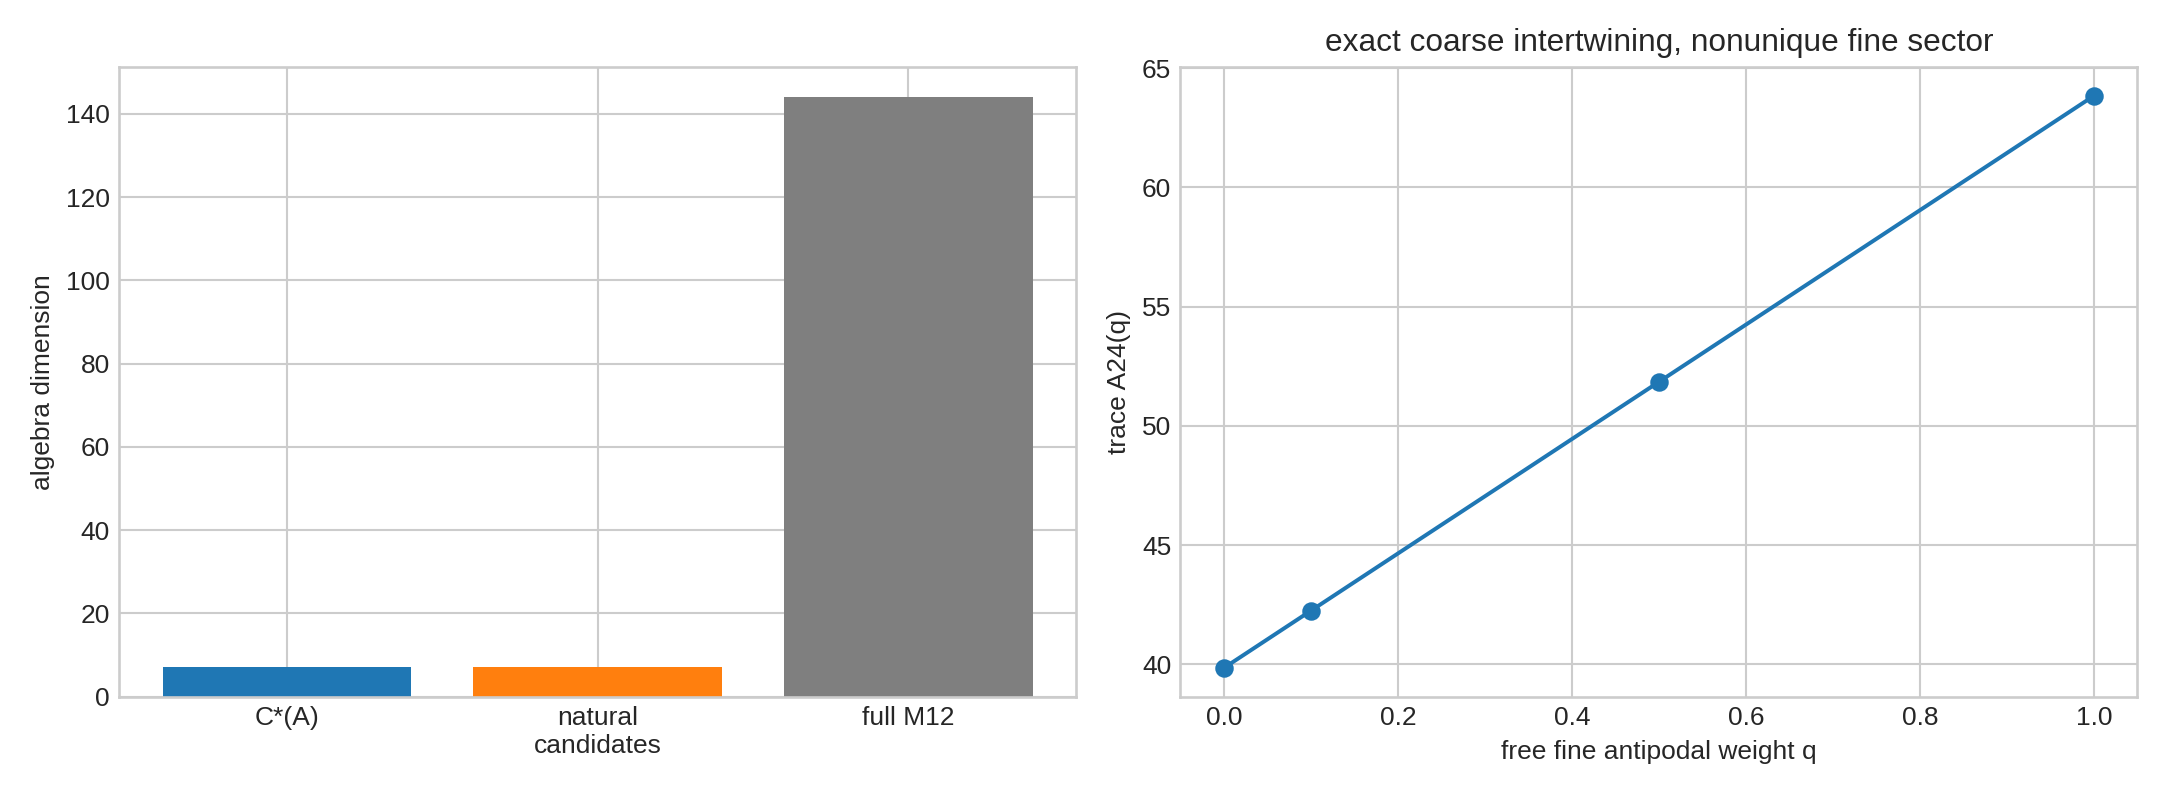
\includegraphics[width=0.94\textwidth]{FIN_ST16_ST27_Figures/st17_algebra_st18_refinement.png}
\caption{Left: the invariant algebra remains seven-dimensional. Right: a free fine-sector parameter changes $A_{24}$ while the coarse intertwining remains exact.}
\end{figure}

\resultbox{\textbf{ST18 verdict.} The continuum obstruction is stronger than endpoint interpolation alone: even an exact, positive, translation-covariant lift has an infinite unresolved fiber. A refinement functor needs an additional coherence or selection axiom.}

\section{ST19 and ST20 --- Derived cross-channel testing with branch control}

\subsection{ST19: a nondefinitional channel identity}

Under the one-generator ansatz $H_{1A}$,
\[
U_tP_\tau=e^{-itA}e^{-\tau A}=e^{-(\tau+it)A}.
\]
This identity is derived from common generation and does not test the analytic strict-kernel formula directly. The observable was frozen as the relative Frobenius residual between the two sides after calibrating $A$ from one heat channel.

The configuration and threshold $10^{-10}$ were serialized and hashed before a 400-case common-generator holdout and a separate 400-case altered-unitary holdout. The hash is
\begin{center}
\texttt{0b4ccd92d5f76f9da87e73aa564cf64bf0bdabb2250e21bc75cf878777fcb838}.
\end{center}
The largest common-generator score is $2.04\times10^{-15}$. The smallest altered-generator score is $5.63\times10^{-4}$. There are no false rejections or false accepts.

\boundary{} This is a better logical prediction than the ST14 formula fingerprint, but remains a local synthetic test. Provider, registrar, analyst, and record custodian are not independent.

\subsection{ST20: scalar interval certificate}

The strict decimal parameters were reevaluated with 55-decimal \texttt{mpmath.iv} interval arithmetic using the exact circulant eigenvalue formula. The certified lower bounds are
\[
\min_{r\ne s}|\lambda_r-\lambda_s|>0.0435757690672,
\]
\[
\pi-0.47\lambda_{\max}>2.04076709425,
\qquad
\pi-0.55\sqrt{\lambda_{\max}}>2.29986225290.
\]
Thus unitary phases are unaliased, the wave arccosine remains on one monotone branch, and heat, Green, Gibbs, and wave scalar spectra uniquely match the seven spectral projectors. The rank-one altered generator has a certified relative separation above $0.0238561$.

\begin{figure}[H]
\centering
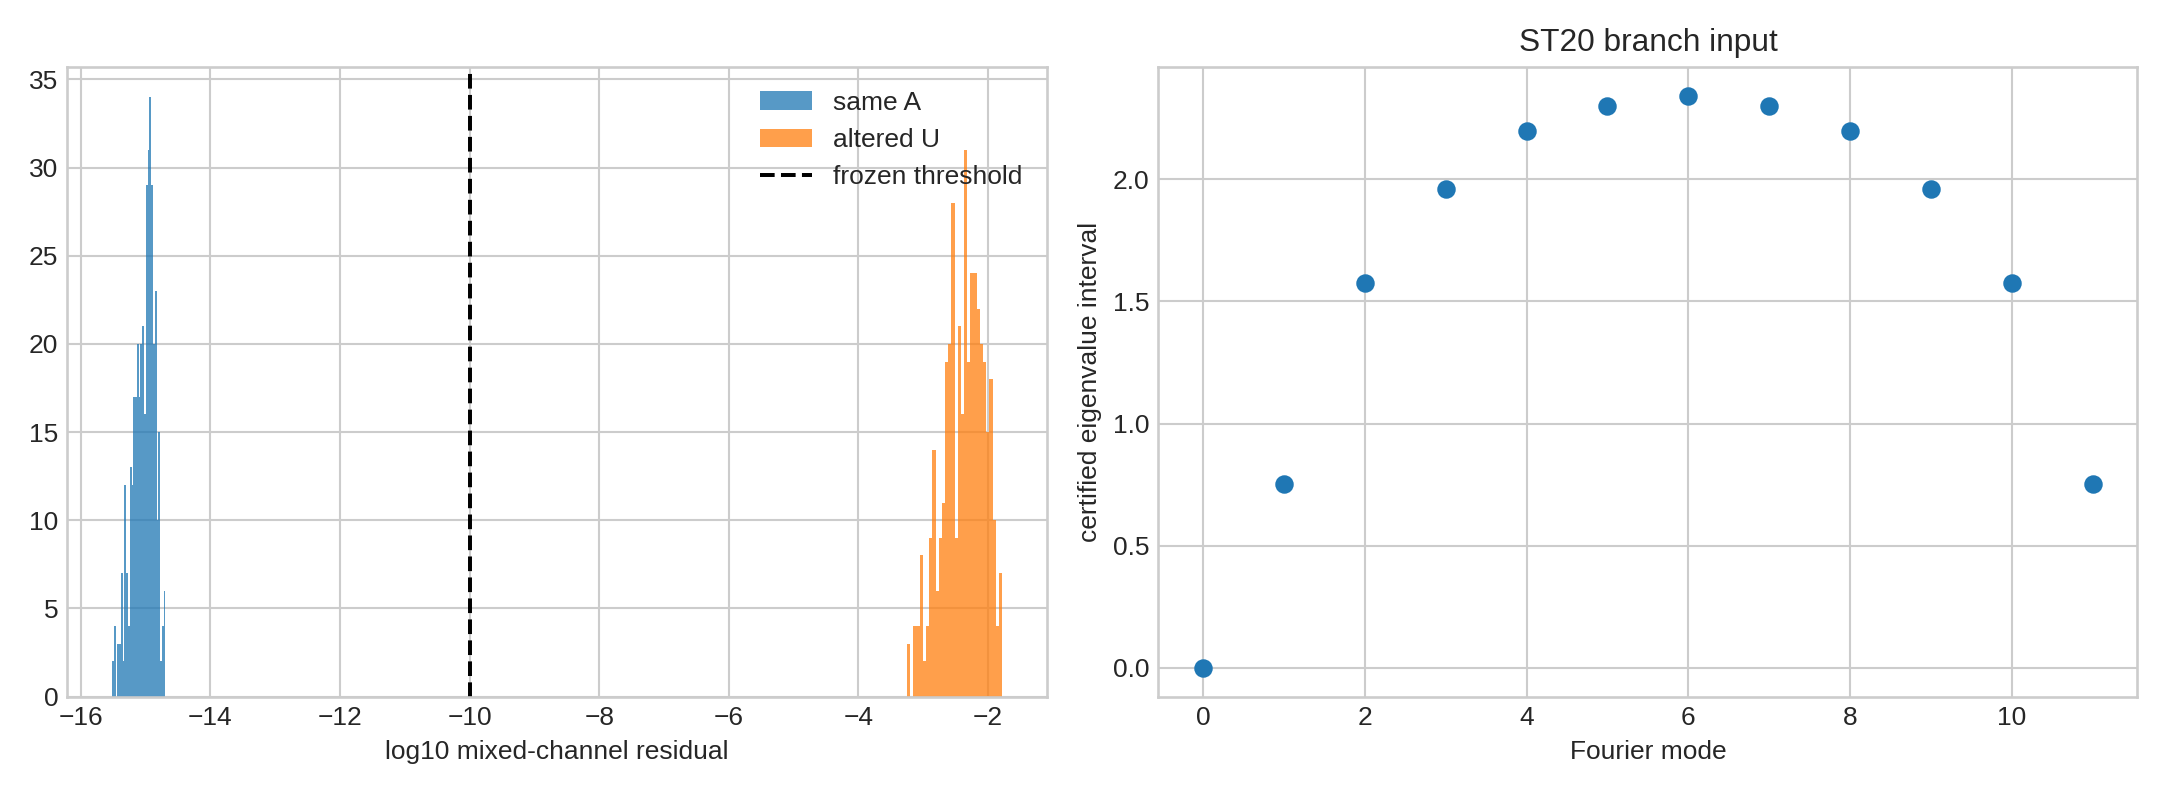
\includegraphics[width=0.94\textwidth]{FIN_ST16_ST27_Figures/st19_prediction_st20_intervals.png}
\caption{Left: the derived mixed-channel holdout. Right: the interval-enclosed Fourier eigenvalues used for branch and projector matching.}
\end{figure}

\boundary{} The interval certificate trusts the implementation of \texttt{mpmath.iv} and is not a proof-assistant verification of transcendental enclosures.

\section{ST21 --- Finite-range path bounds and long-range tails}

\begin{theorem}[Path-order propagation bound]
If $A_{xy}=0$ whenever the cyclic distance exceeds $R$, then every contribution from $x$ to $y$ requires at least
\[
\ell=\left\lceil\frac{d(x,y)}R\right\rceil
\]
off-diagonal steps. Consequently
\[
\left|e^{-itA}_{xy}\right|
\le e^{t\|A\|}\frac{(t\|A\|)^\ell}{\ell!}.
\]
For Hermitian $A$ and $A_R$, Duhamel's formula gives
\[
\|e^{-itA}-e^{-itA_R}\|\le t\|A-A_R\|.
\]
\end{theorem}

The finite $C_{12}$ controls verify the path bound for interaction ranges $R=1,2,3,6$. For the literal $N=192$ continuation, the absolute tail bound decreases with a fitted exponent $-0.843$, close to the envelope expectation $1-\eta=-0.8$. At $R=64$ and $t=0.1$, the actual unitary operator error is $0.00128021$, while the spectral Duhamel bound is $0.001280213$.

\begin{figure}[H]
\centering
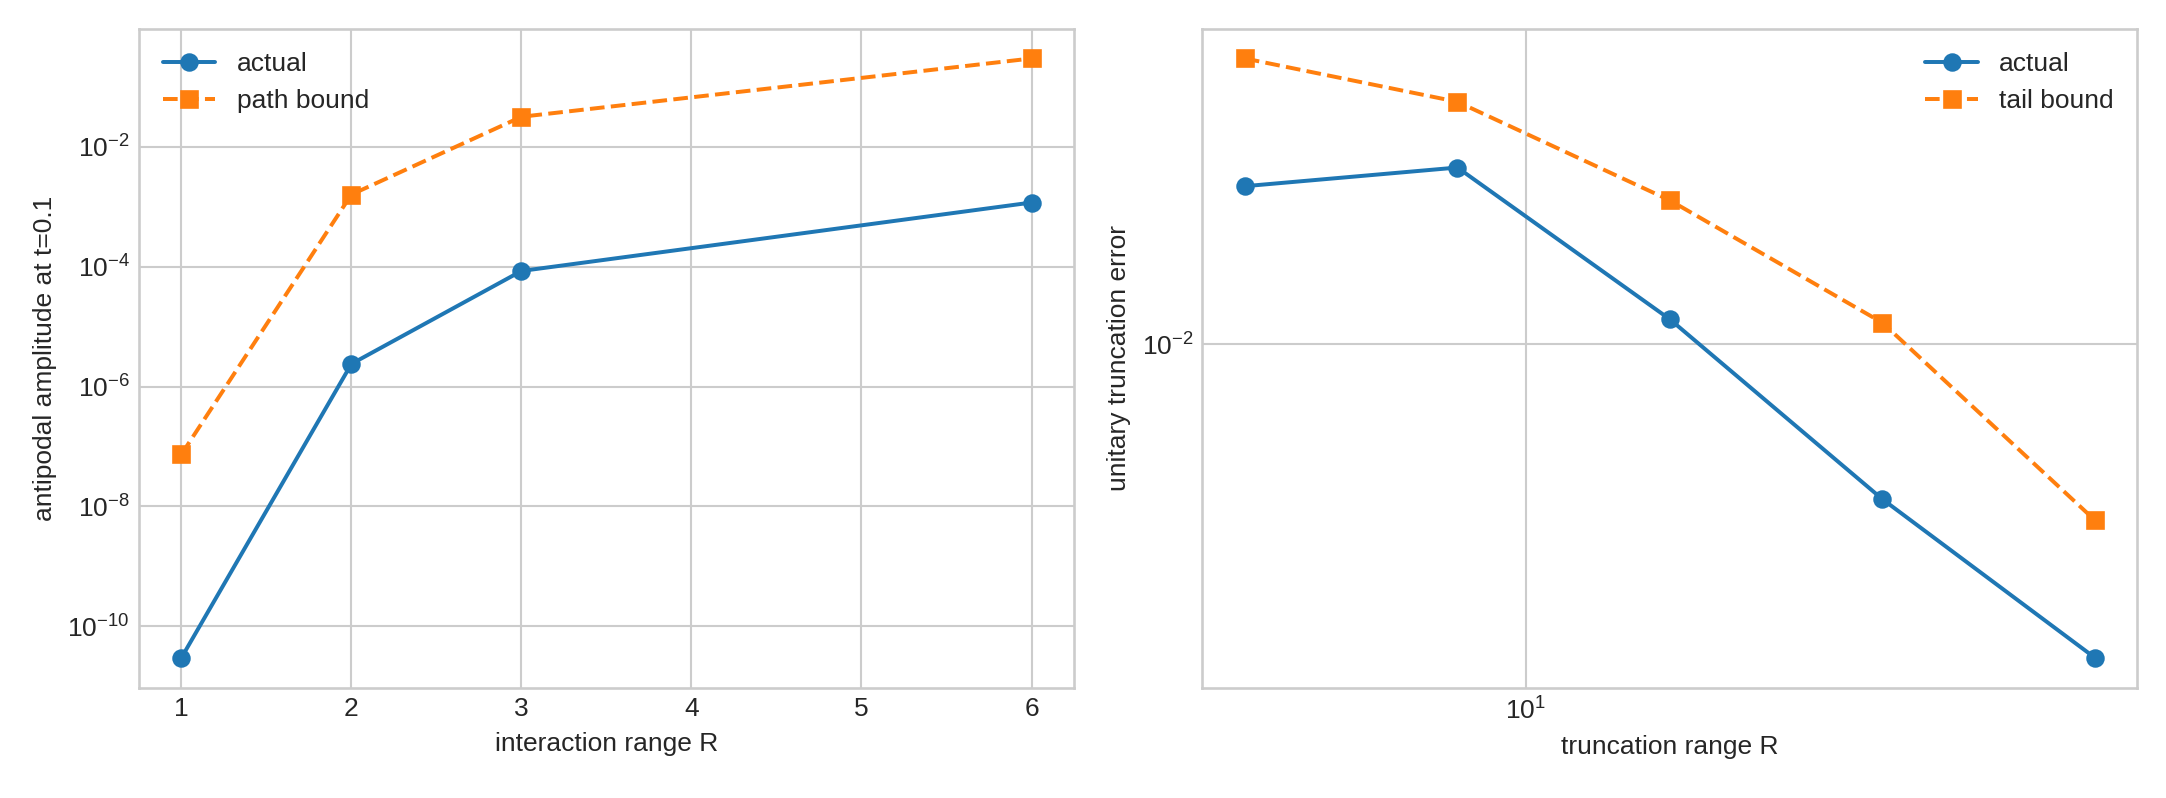
\includegraphics[width=0.94\textwidth]{FIN_ST16_ST27_Figures/st21_locality_bounds.png}
\caption{Conditional locality for finite-range truncations and the polynomial truncation tail of the literal long-range continuation.}
\end{figure}

\boundary{} The literal profile is signed from distance eight. Its Hermitian unitary is valid, but the corresponding heat channel is no longer a Markov transition semigroup. No Lorentzian metric or continuum cone is obtained.

\section{ST22 --- Minimal operational obligations after packaging}

The nine maps listed by ST01 are not all independent mathematical primitives. In an operational process theory:
\begin{itemize}
\item a preparation is a process from the monoidal unit;
\item an observable is an effect or instrument with classical output;
\item an environment can be operationally absorbed into a reduced channel, although its dilations are nonunique;
\item apparatus calibration can be metadata of the instrument context;
\item a probability record can be the classical output of an instrument, while independent custody cannot be generated internally.
\end{itemize}

Relative to this packaging, five obligation groups remain:
\begin{enumerate}
\item sector selection;
\item dimensional calibration;
\item refinement/coarse graining;
\item an operational process theory containing preparations, instruments, outputs, and composition;
\item an external record and custody relation.
\end{enumerate}

Finite countermodels establish independence. Localized and uniform preparations differ by total variation $11/12$ under the vertex measurement. Vertex and Fourier measurements differ by the same amount on a localized state. Independent and perfectly correlated two-bit compositions have the same marginals but total variation $1/2$. The scale orbit has residual zero, and ST18 supplies four explicitly distinct exact lifts.

\boundary{} This is a relative minimality theorem for finite operational semantics, not a claim that every mathematical foundation of physics must use these words.

\section{ST23 --- Connection-source obstruction}

A translation-invariant real $U(1)$ link one-form on $C_{12}$ is determined by five independent coefficients
\[
\theta_d=-\theta_{-d},\qquad d=1,\ldots,5.
\]
The antipodal coefficient vanishes by antisymmetry.

\begin{theorem}[No continuous dihedral-natural connection from $A$]
Reflection maps every coefficient to
\[
\theta_d\longmapsto\theta_{-d}=-\theta_d.
\]
Therefore a reflection-invariant continuous one-form has $\theta_d=0$ for every $d$. Since strict $A$ is reflection invariant, any deterministic stabilizer-equivariant map from $A$ to such a connection returns the zero connection.
\end{theorem}

The exact integer constraint matrix has rank five and invariant nullity zero. Cycle holonomy is reversed by reflection, so fixed fluxes satisfy $\Phi=-\Phi\pmod{2\pi}$, leaving only $0$ and $\pi$.

\resultbox{\textbf{ST23 verdict.} The nonzero flux used in ST08 is necessarily inserted relative to the strict symmetric endpoint. A derived connection requires a new state, boundary, discrete sector, or genuine symmetry-breaking source.}

\section{ST24 --- Coercive saturation universality classes}

Consider the constructed family
\[
q_a(\rho)=\frac{\rho}{(1+\rho/R)^{1-a}},
\qquad
V_a(\rho)=-\frac{g^2}{2b}q_a(\rho)^2+\frac\mu2\rho,
\qquad 0\le a\le1.
\]
Every member has
\[
q_a(\rho)=\rho+O(\rho^2),
\qquad
V_a(\rho)=-\frac{g^2}{2b}\rho^2+O(\rho^3)+\frac\mu2\rho,
\]
and therefore shares the same attractive fourth-order field jet.

\begin{theorem}[Sharp asymptotic coercivity threshold]
As $\rho\to\infty$,
\[
q_a(\rho)^2\sim R^{2-2a}\rho^{2a}.
\]
For $\mu>0$, $V_a$ is coercive if $a<1/2$, is coercive at $a=1/2$ precisely when
\[
\mu>\frac{g^2R}{b},
\]
and is unbounded below when $a>1/2$.
\end{theorem}

\begin{figure}[H]
\centering
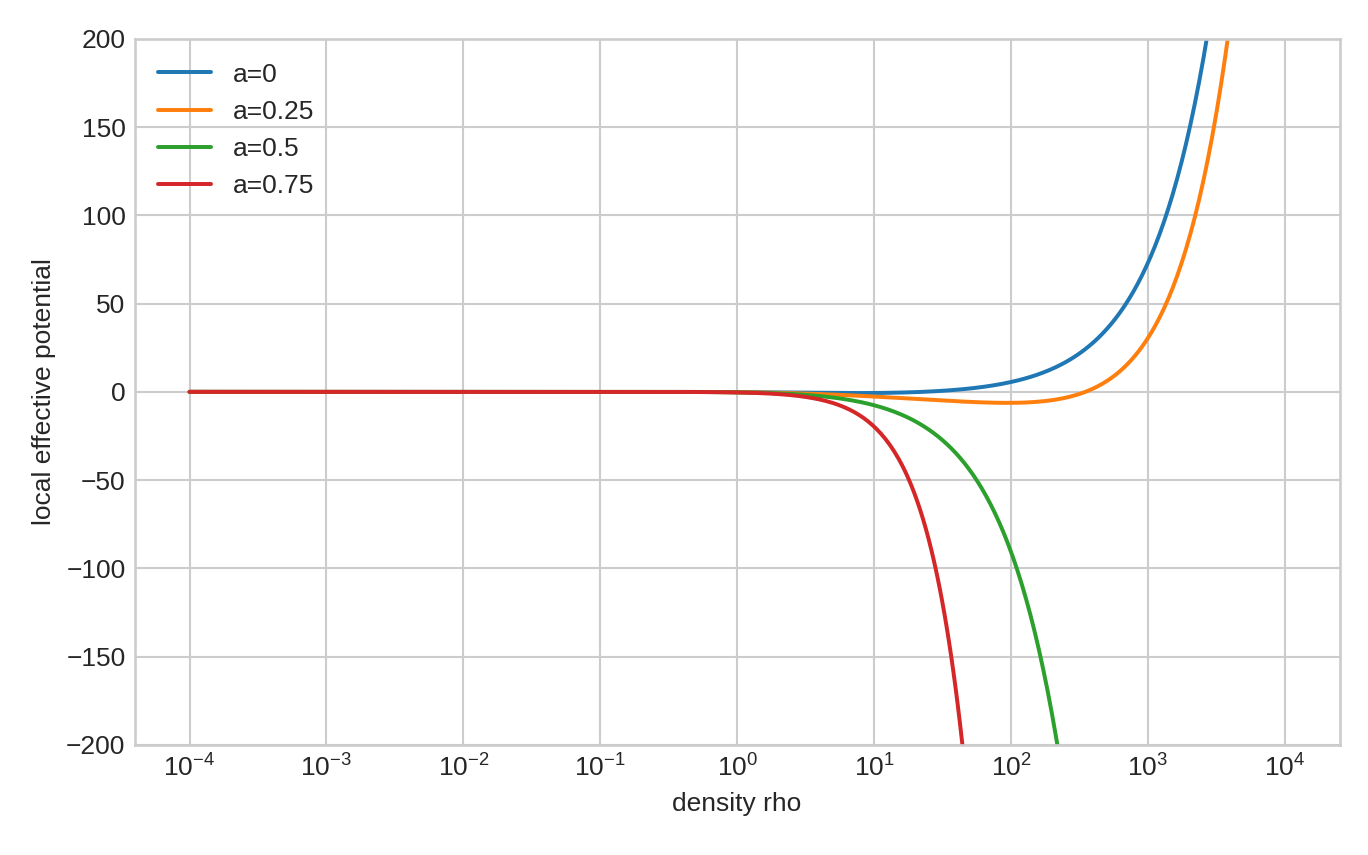
\includegraphics[width=0.78\textwidth]{FIN_ST16_ST27_Figures/st24_saturation_classes.png}
\caption{Potentials sharing the same attractive local jet separate into coercive and noncoercive asymptotic classes.}
\end{figure}

For $(b,g,R,\mu)=(1,1,2,0.15)$, $a=0$ and $a=1/4$ are coercive, while $a\ge1/2$ is noncoercive. This proves that the local attractive jet does not determine global stability.

\boundary{} The saturation function and positive mass term remain added axioms. This classification does not derive a nonlinear FIN law or establish a physical soliton.

\section{ST25 --- Formal replay boundary}

The source \texttt{FIN\_ST25\_Formal\_Core.lean} contains candidate Lean proofs of:
\begin{enumerate}
\item the approximate-shadow composition identity;
\item a three-vertex Dirichlet identity;
\item the thermal scaling orbit;
\item the reversal element in $\operatorname{Aut}(\mathbb Z_{12})$.
\end{enumerate}
Its SHA-256 hash is
\begin{center}
\texttt{11b6ab4cd37de7ecbc876547e7043b982a6d5983d717d4c351d8415129b7a866}.
\end{center}

\blocked{} The \texttt{lean} launcher is present, but no default toolchain is configured. No network installation was attempted. The source is therefore exported but not machine checked. ST25 does not remove the ST15 trust boundary.

\section{ST26 --- Multiweight dimensional equivariance}

The five channels require distinct dimensionless coordinates:
\[
U=e^{-i\alpha_UtA},\qquad P=e^{-\alpha_PtA},\qquad
C=\cos(t\sqrt{\alpha_CA}),
\]
\[
G=(\alpha_GA+zI)^{-1},\qquad
\rho_\beta=\frac{e^{-\beta E_*A}}{Z}.
\]

\begin{theorem}[Multiweight scale orbit]
The channels are equivariant under positive scaling, but with weights
\[
\begin{array}{c|c}
\text{channel}&\text{scale action}\\\hline
U,P&\alpha\mapsto c\alpha,\quad t\mapsto t/c\\
C&\alpha_C\mapsto c\alpha_C,\quad t\mapsto t/\sqrt c\\
G&\alpha_G,z\mapsto c\alpha_G,cz,\quad G\mapsto G/c\\
\rho_\beta&E_*\mapsto cE_*,\quad\beta\mapsto\beta/c.
\end{array}
\]
A single dimension assignment to $A$ cannot make it simultaneously a first-order generator of dimension $T^{-1}$ and a wave stiffness of dimension $T^{-2}$.
\end{theorem}

Thus mode and soliton frequencies can define dimensionless phase time and ratios, but do not produce seconds. Sector maps, a squared-operator relation, or independently calibrated constants are necessary.

\section{ST27 --- Isospectral sector-refit adversaries}

Let $Q$ be an orthogonal matrix fixing the uniform zero mode and define $A_Q=QAQ^T$. Every $A_Q$ has exactly the strict spectrum. A channel generated by $A_Q$ therefore passes all spectrum-only comparisons.

\begin{theorem}[Frozen no-refit principle]
If a channel function $f$ is injective on the certified spectral branch, then
\[
f(B)=f(A)\quad\Longrightarrow\quad B=A
\]
by inverse functional calculus. Hence $f(QAQ^T)$ agrees with $f(A)$ only when $Q$ preserves the relevant spectral projectors. Sector-specific refitting always hides the mismatch by replacing $A$ with $A_Q$.
\end{theorem}

Sixty random stabilizer-fixing rotations were tested at each of nine rotation sizes. Eigenvalue discrepancies remain below $5\times10^{-15}$ and every sector-specific refit is exact to floating precision. With frozen matrix threshold $10^{-3}$, every sample at rotation size $0.01$ or larger is rejected, whereas the smaller declared perturbations are not.

\begin{figure}[H]
\centering
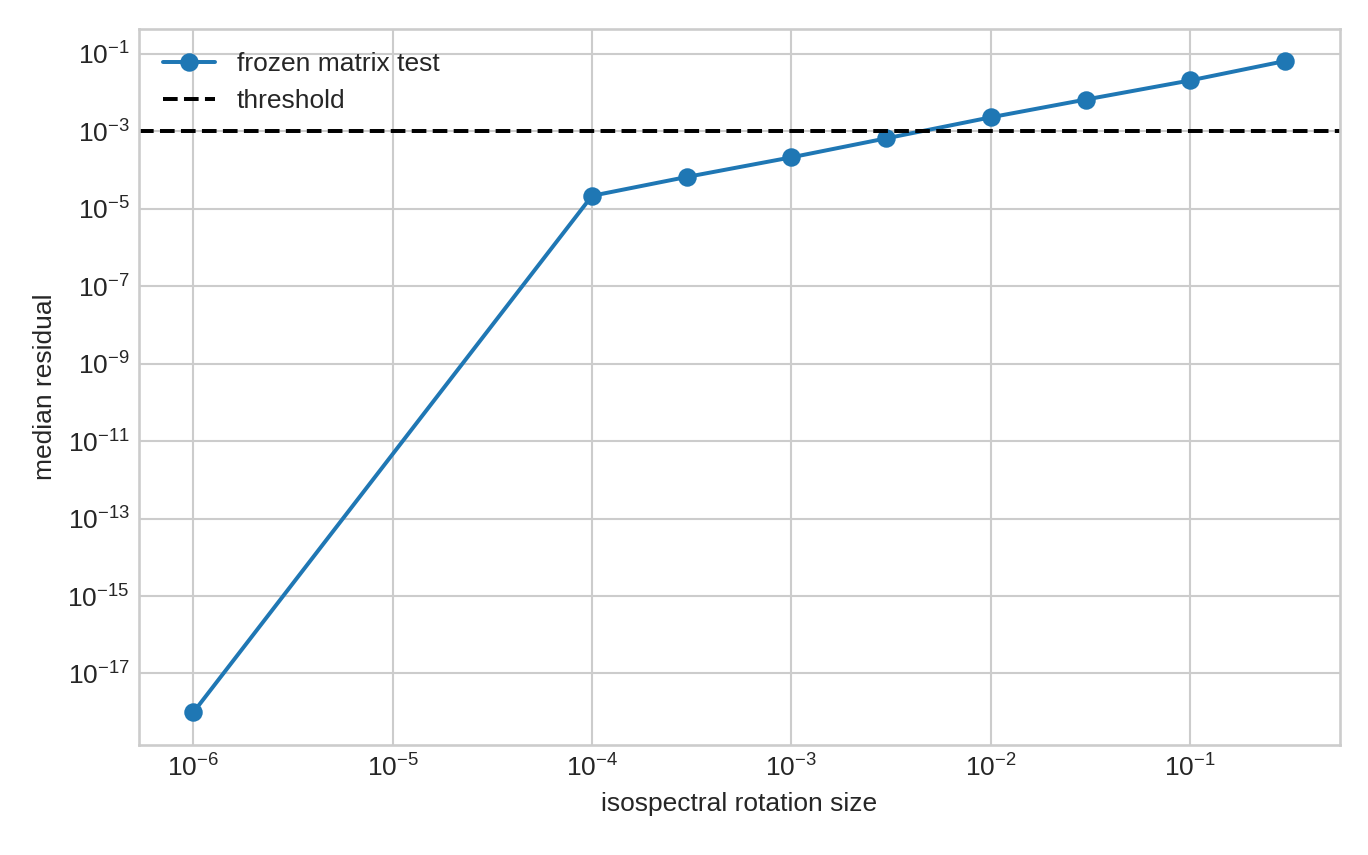
\includegraphics[width=0.78\textwidth]{FIN_ST16_ST27_Figures/st27_adversarial_refits.png}
\caption{Isospectral rotations are invisible to spectrum-only tests but visible to a frozen matrix-level common-generator protocol.}
\end{figure}

\boundary{} Detection thresholds and rotations are synthetic. The program validates protocol logic and does not constitute external evidence for $H_{1A}$.

\section{Synthesis: what changed?}

The batch closes several questions more sharply than ST01--ST15:
\begin{itemize}
\item the Hamiltonian-memory transition is a gauge-Jordan collision governed by one explicit scalar function;
\item invariant information contained in $A$ cannot internally generate the missing noncommutative algebra or an oriented continuous connection;
\item exact positive refinement does not remove continuum ambiguity;
\item locality can be bounded after truncation, but the literal long-range profile is signed and non-Markov;
\item the attractive local nonlinear jet belongs to multiple incompatible global stability classes;
\item common spectral generation is testable only through frozen matrix/projector relations, not eigenvalue matching alone;
\item dimensional physics needs a family of sector-scale maps rather than one universal dimensional reading of $A$.
\end{itemize}

\resultbox{\textbf{Deepest surviving interpretation after ST27.} Strict FIN remains a finite symmetric information-spectral generator. Its exact functional channels, memory realizations, refinements, gauge receivers, and nonlinear completions form a controlled library of mathematical possibilities. The missing physics is the mechanism that selects one state, one refinement, one dimensional calibration, one operational sector, and one externally recorded realization.}

\section{Recommended Programs ST28--ST39}

\begin{longtable}{@{}p{0.08\textwidth}p{0.11\textwidth}p{0.70\textwidth}@{}}
\toprule
ID & Priority & Study and success criterion\\
\midrule
ST28 & 1 & Interval-certify the ST16 stationary branch, Jordan coefficients, and unique collision root.\\
ST29 & 2 & Classify state-dependent and orbit-valued symmetry breaking outside the ST17 invariant no-go.\\
ST30 & 3 & Impose refinement associativity on the ST18 fiber and classify dyadic natural transformations.\\
ST31 & 4 & Add finite counts and a frozen likelihood to the derived ST19 cross-sector observable.\\
ST32 & 5 & Prove long-range polynomial propagation bounds for $\eta=1.8$ without Markov semantics.\\
ST33 & 6 & Classify discrete $\pi$ holonomy and state-sourced connections permitted by ST23.\\
ST34 & 7 & Prove existence and orbital stability for the coercive ST24 saturating DNLS family.\\
ST35 & 8 & Configure a pinned offline Lean toolchain and replay ST25.\\
ST36 & 9 & Derive identifiability conditions for all ST26 sector scales.\\
ST37 & 10 & Add finite-count noise and nuisance calibration to the ST27 adversarial protocol.\\
ST38 & 11 & Search for a strict-sourced non-invariant state jointly addressing selector, connection, and algebra.\\
ST39 & 12 & Build a consolidated theorem-dependency graph for ST01--ST27 and identify the minimal independent axioms.\\
\bottomrule
\end{longtable}

\section{Final verdict}

ST16--ST27 do not turn FIN into physics. They produce three exact obstruction layers:
\begin{enumerate}
\item stabilizer-invariant functions of $A$ cannot supply the selector or oriented connection;
\item exact positive coarse intertwining does not select a refinement;
\item a single dimension assignment cannot serve all spectral channels.
\end{enumerate}
They also produce one analytically reduced dynamical mechanism, one sharp nonlinear coercivity classification, interval branch control, and stronger synthetic falsification protocols.

The correct next scientific priority is ST28: certify the Jordan collision with validated stationary-state and coefficient intervals. In parallel, ST30 should determine whether multiscale associativity reduces the exact ST18 refinement fiber. Neither direction licenses a physical or ToE claim before operational and external-evidence obligations are met.

\appendix
\section{Reproduction}

\begin{verbatim}
MPLCONFIGDIR=/tmp/fin-st16-mpl python3 fin_st16_st27_research.py
MPLCONFIGDIR=/tmp/fin-st16-test-mpl \
  python3 -m unittest -v test_fin_st16_st27.py
pdflatex -interaction=nonstopmode -halt-on-error \
  FIN_ST16_ST27_Selectors_Refinement_and_Dimensional_Bridge_Report_EN.tex
sha256sum -c FIN_ST16_ST27_RELEASE_MANIFEST.sha256
\end{verbatim}

The deterministic run writes JSON, CSV, six figures, a cross-sector preregistration record, and a scalar interval certificate. Fifteen live acceptance tests pass.

\section{Internal provenance and trust boundaries}

ST16 continues the P530/ST10 Hamiltonian-memory family. ST17--ST23 continue the selector, continuum, prediction, interval, locality, operational, and gauge questions defined by Release 10.55. ST24 extends the constructed ST09/P527 mediator family. The principal upstream artifacts are:
\begin{itemize}
\item \texttt{FIN\_ST01\_ST15\_Shadow\_to\_Physics\_Bridge\_Research\_Report\_EN.pdf};
\item \texttt{FIN\_ST01\_ST15\_Results.json};
\item \texttt{FIN\_Programs\_527\_536\_Results.json};
\item the kernel provenance and strategic guardrail packets listed in \texttt{FIN\_ST16\_ST27\_INPUTS.sha256}.
\end{itemize}

The memory collision and adversarial curves use binary64 linear algebra. ST20 trusts \texttt{mpmath.iv}. ST25 is not machine checked. All prediction records remain locally generated and synthetic.

\section{Scope and non-claims}

This release does not discharge QW-2191, select canonical orientation, source a physical clock or units, construct a unique continuum, derive a gauge field, derive a nonlinear FIN law, complete the legacy-to-strict bridge, transfer any legacy physical role, provide apparatus, create independent custody, add laboratory data, derive the Standard Model or gravity, construct $L_{\rm total}$, or establish a Theory of Everything.

\end{document}
